% (c) Egor Osipov

\documentclass[a4paper,12pt]{article} % тип документа (report, book)
\usepackage[14pt]{extsizes}
\usepackage[left=2cm,right=2cm, top=2cm,bottom=2cm,bindingoffset=0cm]{geometry} % Настройки документа


%  Русский язык
\usepackage[T2A]{fontenc}			% кодировка
\usepackage[utf8]{inputenc}			% кодировка исходного текста
\usepackage[english,russian]{babel}	% локализация и переносы


% Математика
\usepackage{amsmath,amsfonts,amssymb,amsthm,mathtools} 

% Просто смайлики
\usepackage{wasysym}

%Вставка картинок
\usepackage{graphicx}
\graphicspath{./}
\DeclareGraphicsExtensions{.pdf,.png,.jpg}
\usepackage{float}

% Настройка абзацев
\usepackage{indentfirst}
%\setlength{\parindent}{5ex}
%\setlength{\parskip}{1em}

\begin{document} % начало документа

%Заговолок
\begin{titlepage}
\begin{center}
	\large{Московский физико-технический институт}\\
	\vspace{100px}
	\LARGE{Лабораторная работа № 3.2.2}\\
	\LARGE{Резонанс напряжений.}\\
	\vspace{30px}
	
\includegraphics[scale = 0.3]{fakt_logo.png}\\
\end{center}

\vfill
\begin{flushright}
	\text{Осипов Егор. Б03-005}\\
	\text{07.09.2021}\\
	\text{г. Долгопрудный}
\end{flushright}
\end{titlepage}

\newpage

\tableofcontents

\newpage

\newpage

\section{Предстоит сделать.}
\subsection{Цель работы и оборудование.}

\textbf{Цель работы:} Изучение последовательной цепи переменного тока, наблюдение резонанса напряжений. Определение добротности и сопротивления контура,а так же параметров катушки.

\textbf{В работе используется:} Регулировочный трансформатор, катушка индуктивности с выдвижным сердечником, магазин емкостей, реостат, резистор, амперметр, три вольтметра, ваттметр, осциллограф, универсальный мост.

\section{Теоритические сведения.}

\subsection{Теория, как она есть.}

Все колебания рассмотриваются в условиях \textbf{квазистационарности}. Это означает, что мгновенные значения тока I практически одинаковы во всех проводниках, соединяющих элементы цепи, а изменения во времени происходят настолько медленно, что распространение электродинамических взаимодействий можно считать мгновенным.

Это позволяет нам пользоваться ЗСЗ и законом Ома для замкнутой цепи для цепей перемнного тока. Отсюда следуют и \textbf{правила Кирхгофа}. Первое: алнебраическая сумма токов в узле равна нулю. Второе: для любого замкнутого контура сумма падений напряжений на отдельных участках контура равна алгебраической сумме ЭДС в этом контуре.

Используя правила Кирхгофа для цепей перменного тока, мы получаем систему линейных дифференциальных уравнений, которые позволяют найти \textit{временную} зависимость токов в данной цепи.

\subsection{Свободные колебания}

Сумма падений напряжений в цепи равна ЭДС самоиндукции катушки:

\begin{equation}\label{2.4}
RI + U_C = -L \frac{dI}{dt};\;\;\;
L \frac{dI}{dt} + RI + \frac{q}{C}
\end{equation}

\begin{equation}\label{2.6}
L \frac{d^2 I}{dt^2} + R \frac{dI}{dt} + \frac{I}{C} = 0
\end{equation}

Разделим уравнение на L и введем обозначения:

\begin{equation}\label{2.7}
\gamma = \frac{R}{2L}; \;\;\;\;\;  \omega^2_0 = \frac{1}{LC}
\end{equation}

Таким образом получаем $\gamma$ - \textbf{коэффициент затухания} и $\omega_0$ - \textbf{собственная частота} контура.

Подобными уравнениями описывают целый ряд колебательных систем. Проще всего иъ представить в виде уравнения:

\begin{equation}\label{2.9}
I = A \cdot e^{\lambda t}
\end{equation}

От этого вида уравнения можно простой подстановкой перйти в \textbf{характеристическому} виду уравнения:

\begin{equation}\label{2.10}
\lambda^2 + 2\gamma \lambda + \omega^2_0 = 0
\end{equation}

Величина $\omega = \sqrt{\omega^2_0 - \gamma^2}$ называется \textit{частотой свободных колебаний}.

\subsection{Свободные колебания. Метод комплексных амплитуд.}

Так называют контур, в котором ЭДС изменяется по гармоническому закону:

\begin{equation}\label{2.00}
\varepsilon = \varepsilon_0 \cos(\Omega t)
\end{equation}

\begin{figure}[H]
\noindent\centering{
\hspace{-0mm}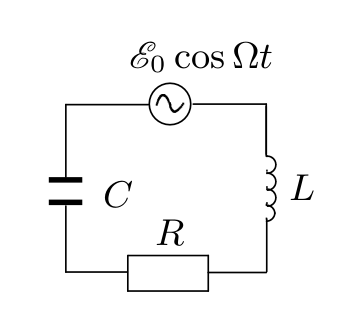
\includegraphics[scale=0.5]{theory1}
}
\caption{Последовательный контур с внещним ЭДС.}
\label{pic0:ref}
\end{figure}

\subsection{Свободные колебания. Резонанс.}

Снова рассмотрим процессы протекающие в последовательном контуре \eqref{pic0:ref} подсоединенном к внешней ЭДС. Продивверенцируем уравнени из лабника (2.34) по времени:

\begin{equation}\label{2.44}
L \frac{d^2I}{dt^2} + R \frac{dI}{dt} + \frac{1} {C} I = -\varepsilon_o \Omega \sin(\Omega t)
\end{equation}

Находя общее решение однородного уравнения $I_1$ и любое частное решение $I_2$ найдем решение дифференциального уравнения, полученного заменой $\sin(\Omega t)$ на $e^{i \Omega t}$ и разделением уравнения \eqref{2.44} на L.

\subsection{Формулы и зависимости.}

\noindentВыражение для напряжения на резисторе, катушке и суммарного напряжения.
\begin{equation}
U_R = IR,\;\;\;\;\;\;U_L = I(r_L + i\Omega L),\;\;\;\;\;\;U_{R+L} = I(R + r_L + i\Omega L)
\label{eq1:ref}
\end{equation}
\noindentГде $r_L$ - активное сопротивление катушки.

\noindentПереходя к модулям и фазам токов и напряжений, найдем из (\ref{eq1:ref}).
\begin{equation}
U_R = IR,\;\;\;\;\;\;\;\;\;tg\varphi_1 = 0
\label{eq2:ref}
\end{equation}

\begin{equation}
U_L = I\sqrt{r_L^2 + (\Omega L)^2},\;\;\;\;\;\;\;\;\;tg\varphi_2 = \frac{\Omega L}{r_L}
\label{eq3:ref}
\end{equation}

\begin{equation}
U_{R+L} = I\sqrt{(R + r_L)^2 + (\Omega L)^2},\;\;\;\;\;\;\;\;\;tg\varphi_3 = \frac{\Omega L}{R + r_L}
\label{eq4:ref}
\end{equation}
\noindentВ этих формулах U и I - эффективные значения напряжения и тока.

\noindentМощность переменного тока, выделяемая в катушке
\begin{equation}
P_L = U_L I cos\varphi = I^2r_L
\label{eq5:ref}
\end{equation}

\noindentВ контуре, настроенном в резонанс на частоту $\Omega$ внешнего источника (собственная частота контура и внешняя совпадают $\omega_0 = \Omega$), реактивные сопротивления индуктивности и емкости одинаковы.
\begin{equation}
\omega_0 L = \frac{1}{\omega_0 C}
\label{eq6:ref}
\end{equation}

\noindentОпределив добротность контура Q, можно рассчитать полное сопротивление контура $R_\Sigma$ в резонансе, поскольку
\begin{equation}
Q = \frac{\omega_0 L}{R_\Sigma} = \frac{1}{\omega_0 C R_\Sigma}
\label{eq7:ref}
\end{equation}

\begin{equation}
R_\Sigma = R + r_L
\label{eq8:ref}
\end{equation}

\noindentРезонанстные напряжения на контуре и на емкости равны
\begin{equation}
U_{\Sigma\text{рез}} = I_{\text{рез}}R_\Sigma,\;\;\;\;\;\;\;\;\;U_{C\text{рез}} = \frac{I_{\text{рез}}}{\Omega C}
\label{eq9:ref}
\end{equation}

Из (\ref{eq7:ref}) и (\ref{eq9:ref}) получим
\begin{equation}
Q = \frac{U_{C\text{рез}}}{U_{\Sigma\text{рез}}}
\label{eq10:ref}
\end{equation}

\subsection{Экспериментальная установка}

\begin{figure}[H]
\noindent\centering{
\hspace{-0mm}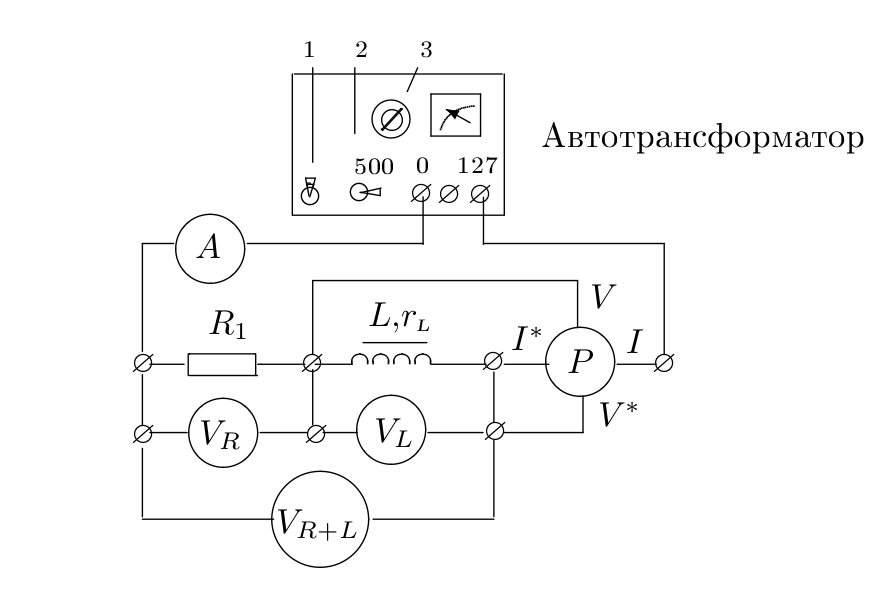
\includegraphics[scale = 0.5]{ustanovka1}
}
\caption{Схема установки для изучения закона Ома в цепи переменного тока.}
\label{pic2:ref}
\end{figure}

\begin{figure}[H]
\noindent\centering{
\hspace{-0mm}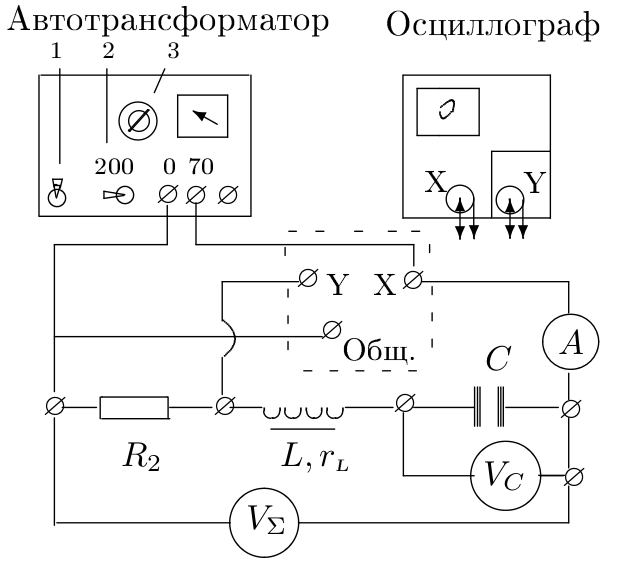
\includegraphics[scale = 0.5]{ustanovka2}
}
\caption{Схема установки для наблюдения резонанса напряжений.}
\label{pic2:ref}
\end{figure}

\newpage

\section{Экспериментальные данные и их обработка.}

\begin{table}[H]
\caption{\label{tab:canonsummary} Данные эксперимента и рассчетные $r_l$ и $L$.}
\begin{center}
\begin{tabular}{|c|c|c|c|c|c|c|c|}
\hline
x(мм) & I(А) & $V_R$(B) & $V_{R+L}$(B) & $V_L$(B) & P(Вт) & $r_l$(Ом) & L(Гн)\\
\hline
5 & 0.80 & 70 & 106 & 70 & 9.25 & 14.45 & 1.73 \\
\hline
7 & 0.85 & 74 & 104 & 63 & 8.25 & 11.42 & 1.46 \\
\hline
9 & 0.88 & 78 & 104 & 58 & 7.75 & 10.12 & 1.31 \\
\hline
11 & 0.93 & 81 & 103 & 53.5 & 7.25 & 8.47 & 1.14 \\
\hline
13 & 0.95 & 83 & 103 & 50 & 7.00 & 7.76 & 1.04 \\
\hline
15 & 0.95 & 84 & 103 & 47 & 6.75 & 7.48 & 0.98 \\
\hline
17 & 0.98 & 85 & 102 & 45 & 6.50 & 6.84 & 0.91 \\
\hline
19 & 0.98 & 86 & 102 & 42 & 6.25 & 6.57 & 0.85 \\
\hline
20 & 0.98 & 86 & 102 & 41 & 6.00 & 6.31 & 0.83 \\
\hline
16 & 0.95 & 84 & 102 & 46 & 6.50 & 7.20 & 0.96 \\
\hline
12 & 0.93 & 82 & 103 & 51 & 7.25 & 8.47 & 1.09 \\
\hline
8 & 0.88 & 76 & 105 & 60 & 8.25 & 10.78 & 1.35 \\
\hline
6 & 0.83 & 72 & 106 & 66 & 9.00 & 13.22 & 1.58 \\
\hline
\end{tabular}
\end{center}
\label{table1:ref}
\end{table}

По данным таблицы построим график зависимости сопротивления катушки $r_L$ и ее индуктивности $L$ от величины смещения сердечника $x$.

\begin{figure}[H]\label{rlx}
	\center{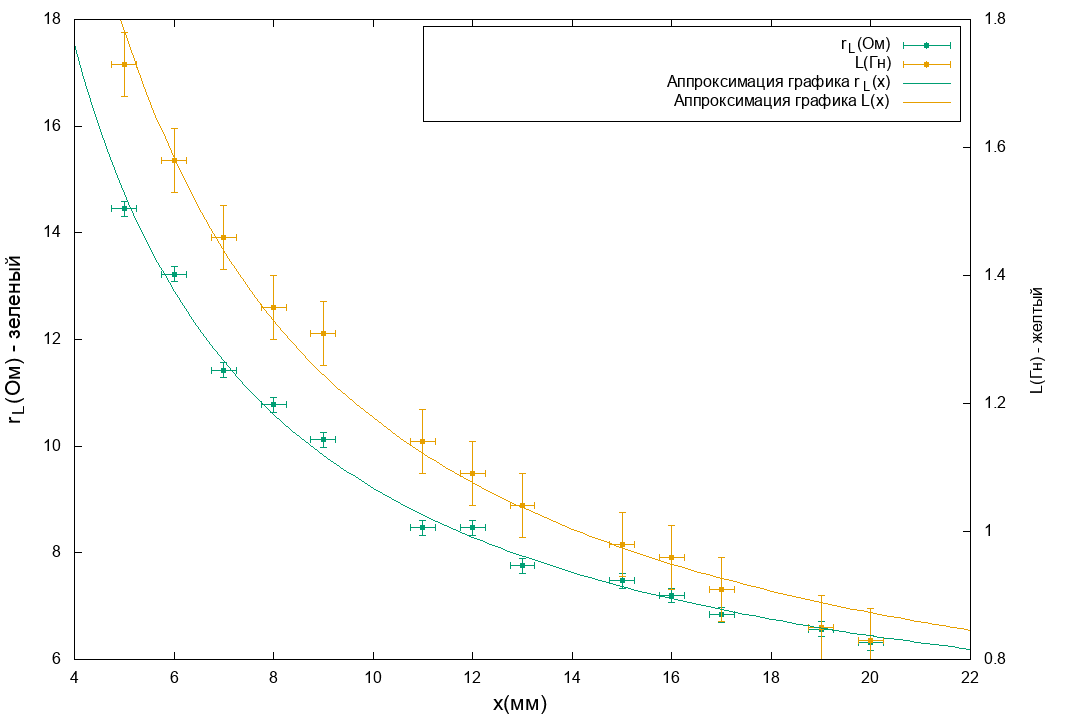
\includegraphics[scale=0.6]{1st_graph}}
%	\caption{}
\label{fig:image}
\end{figure}

Из графика для среднего положения найдем $r_L = 7.37 \pm 0.14\text{Ом}$ и\\ $L = 0.98 \pm 0.05 \text{Гн}$

\begin{figure}[H]\label{vec_diog}
	\center{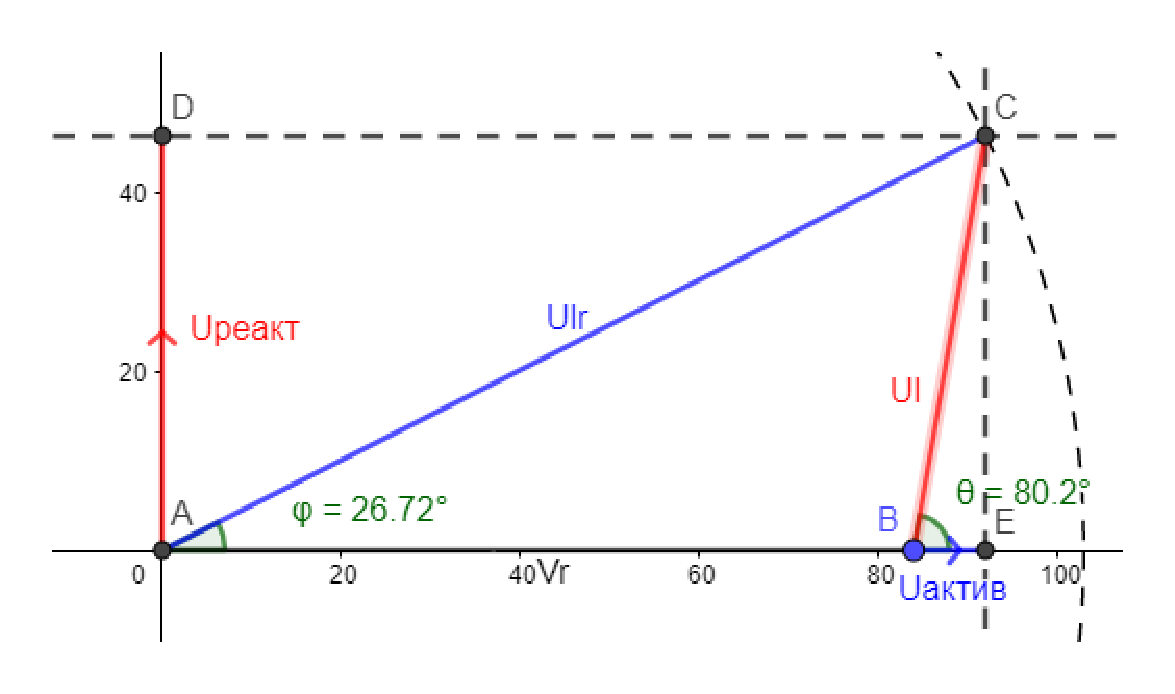
\includegraphics[scale=0.8]{2nd_graph}}
	\caption{Векторная диаграмма напряжений.}
\label{fig:image}
\end{figure}

Из векторной диаграммы найдем (\ref{pic2:ref}): $U_{\text{L,акт}} = 8 \pm 0.5$ (В)  и $U_{\text{L,реакт}} = 46.31 \pm 0.5$ (В). Отсюда:
$$L = \frac{U_{L\text{,реакт}}}{I\Omega} = 0.97\pm 0.01\;\text{Гн}\;\;\;\;\;\;r_L = \frac{U_{L\text{,акт}}}{I} = 7.89\pm0.5\;\text{Ом}$$
Из этой же диаграммы $cos\;\Theta = 0,13$. Теоритический рассчет показывает, что $cos\;\Theta^* = \frac{P_L}{U_L I} = 0.15$. Отличие составляет 16\%.\\

По теореме косинусов
$$P_L = U_L \frac{U_R}{R_1}cos\;\Theta = 5.64\;\;\text{Вт}$$
Отличие от экспериментального значения $P_L^* = 6.75$ Вт составило 16.4\%.\\

Активное сопротивление катушки вычисляем по формуле:

$$r_L = \frac{U_{\Sigma\text{,рез}} - I_\text{рез}\cdot R_2}{I_\text{рез}}$$

Для среднего положения: $r_L = 4.28\pm0.21$ Ом.\\

Условия резонанса: 
$$\omega_0 = 2\pi \nu \;\;\;\;\;\;\; L = \frac{1}{\omega^2 C} \;\;\;\;\;\;\; r_L = \frac{\omega_0 L}{Q}$$

Для среднего положения: L = 0.17 Гн, $r_L = 4.15$ Ом.

Полученные значения сведем в таблицу:

\begin{table}[H]
\begin{center}
\begin{tabular}{|c|c|c|c|c|c|}
\hline
$\;$ & График & Векторная диаграмма & Резонанс & Добротность & LCR-метр\\
\hline
$r_L \text{Ом}$ & $7.37\pm0.14$ & $7.89\pm0.5$ & $4.28\pm0.21$ & 4.15 & 3.28\\
\hline
L Гн & $0.98\pm0.05$ & $0.97\pm0.01$ & -- & 0.17 & 0.13\\
\hline
\end{tabular}
\caption{\label{tab:canonsummary} Итоговые значения индуктивности L и сопротивления $r_L$ катушки}
\end{center}
\label{table2:ref}
\end{table}

\section{Вывод.}

Получены значения сопротивления $r_L$ и индуктивности L катушки (таблица \eqref{tab:canonsummary}). Добротность составила 5.52. Расхождения результатов первых двух от последующих ихмерений обусловлены скорее всего тем, что при выполнении лабораторной работы мы с другими выполняющими обменялись катушками (ненамеренно).

\end{document}